In diesem Abschnitt werde ich zunächst den HOG2D aus \cite{dalal2005histograms} kurz vorstellen, mit dem Hauptthema HOG3D fortfahren und zuletzt das in \cite{scherer2010histograms} durchgeführte Experiment aufgreifen.

\subsection{HOG2D}
Im Bereich der 2D Objekterkennung aus Bildern existieren bereits erfolgreiche Methoden. Der Skale-Invariant-Feature-Transform Algorithmus (SIFT),genauere Beschreibung z.B. in \cite{Priese15}
zu finden, arbeitet mit aggregierten Gradienten. Beim HOG2D werden hingegen die Gradienten entsprechend
ihrer Richtung in Histogrammen eingeordnet.
\newline
Die Idee hinter dem HOG2D ist, dass sich Form und Aussehen von Objekten mit Gradienten beschreiben lassen.
Dies ist selbst möglich ohne die genaue Position der Gradienten zu kennen. Der HOG2D läuft grob nach folgenden Schema ab. Zuerst werden die Farbwerte des Bilds,auf dem die Detektion durchgeführt wird, normalisiert. Danach wird das Bild in gleich große, rechteckige Zellen aufgeteilt. Dabei können einzelne Zellen überlappen. Für jede dieser Zellen werden Histogramme für die jeweils berechneten Gradienten angelegt. Die Einteilung erfolgt entsprechend ihrer Richtung. Die Ergebnisse müssen normalisiert werden. Die HOGs werden mittels Detektionsfenster extrahiert und an eine Support Vector Machine (SVM) weitergeben. Danach kann entschieden werden, ob das entsprechende Objekt gefunden wurde. Im Fall von \cite{dalal2005histograms} Menschen. In dem eben genannten Wissenschaftlichen Artikel hat sich durch Experimente herausgestellt, dass die einfache Ableitungsmaske \ref{Abl_Maske} zur Berechnung der Gradienten die besten Ergebnisse liefert. 
Es wurden andere Ableitungsfilter, wie z.B. der Sobel-Operator (Formel \ref{Sobel}, entnommen aus \cite{Priese15}), jedoch waren die Ergebnisse eher enttäuschend. 

\begin{align}
\label{Sobel}
	S_x =	\begin{bmatrix}
				-1 & 0 & 1 \\
				-2 & 0 & 2 \\
				-1 & 0 & 1 
			\end{bmatrix}  &  
	S_y =	\begin{bmatrix}
				-1 & -2 & -1 \\
				 0 & 0 &   0 \\
				 1 & 2 &   1 
			\end{bmatrix}	
\end{align}
Auch wurde, zwecks Optimierung, mit Gaußfiltern experimentiert. Eine Performenceverbesserung wurde ebenfalls nicht erzielt. 
Detailliertere Informationen über den HOG2D sind in \cite{dalal2005histograms} zu finden.

\subsection{HOG3D}


\subsubsection{Erweiterung des HOG2D auf HOG3D}
Der erste Schritt, die Berechnung der Gradienten, erweist sich bei der Erweiterung auf HOG3D ein wenig komplizierter. Zunächst Benötigt man eine Notation für Nachbarschaft und Intensität für die Polygon Meshs. In \cite{scherer2010histograms} wird dafür ein dreidimensionales euklidisches 
Distanzfeld berechnet. Dieses Feld ist als eine reellwertige Funktion aufzufassen, welche auf einem diskreten, regulären 3D Gitter definiert ist. Das Gitter umfasst dabei das komplette Volumen des Meshs \cite{scherer2010histograms}. Die jeweiligen Gitterzellen können auch als Voxel bezeichnet werden. Jeder Voxel enthält dabei die Information über den Abstand seines Zentrums zur Oberfläche des Meshs. 

\begin{equation*}
f: \mathbb{N} \times \mathbb{N} \times \mathbb{N} \mapsto \mathbb{R} 
\end{equation*}
\begin{equation}
\label{Distanzfeld_Fkt}
f(x,y,z) = \min_{\substack{x \in \Sigma}} \| x-center(x,y,z) \|_2
\end{equation}
Eine Definition der Funktion ist bei Formel \ref{Distanzfeld_Fkt} zu sehen, entnommen aus \cite{scherer2010histograms}. $\Sigma$ ist hierbei die Menge aller Punkte auf der Oberfläche des Meshs und $center: \mathbb{N} \times \mathbb{N} \times \mathbb{N} \mapsto p $ liefert die Koordinate des Zentrums des Voxels zurück.
\newline
Auf das berechnete Distanzfeld kann man z.B. die Filtermaske $\begin{bmatrix} -1 & 0 & 1\end{bmatrix}$ aus \cite{dalal2005histograms} anwenden für Die Gradientenberechnung.
\newline
Das Distanzfeld wird sehr stark von Position und große des Objekts beeinflusst. Dementsprechend muss das Mesh vor der Distanzfeldberechnung normalisiert werden. In \cite{scherer2010histograms} greift man deshalb auf Translationsinvarianz  (das Zentrum der Masse des Meshs wird in den Ursprung verlegt), Skalierungsinvarianz (Skallierung des Meshs in den Einheitswürfel), sowie eine Normalisierung für Rotation mittels gewichteter PCA analyse.
\newline
Der zweite Schritt ist im weiten simpler. Die dreidimensionalen Gradienten werden jeweils entsprechend ihrer Richtung in Histogramme für die einzelnen Zellen eingeordnet. Hierfür werden die Gradienten in sphärische Koordinaten entsprechend Formel \ref{Sphere_Koord}, entnommen aus \cite{scherer2010histograms}, umgerechnet.

\begin{equation}
\label{Sphere_Koord}
\begin{pmatrix}
	\theta \\ 
	 \phi \\ 
	 r
\end{pmatrix}
= \begin{pmatrix}
	\arccos\dfrac{z}{\sqrt{x^2+y^2+z^2}} \\ 
	 atan2(x,y) \\ 
	 \sqrt{x^2+y^2+z^2}
\end{pmatrix}
\end{equation}
Die Einordnung erfolgt entsprechend ihrer Richtung ($Zenit \theta \in [0,\pi) $ und $Azimut \phi \in [0,2\pi)$)  

\subsubsection{HOG3D Extraktionsalgorithmus }
Der schematische Ablauf des Extraktionsalgorithmus ist in \figurename~\ref{Vekt_ext_pipe} zu sehen. Genaueres über die Implementation ist in dem in \cite{scherer2010histograms} mitgelieferten Sourcecode \footnote{www.gris.informatik.tu-darmstadt.de/projects/vsa/3dhog/3dhog.zip} zu entnehmen 

 \begin{figure}[thpb]
 	\centering
 	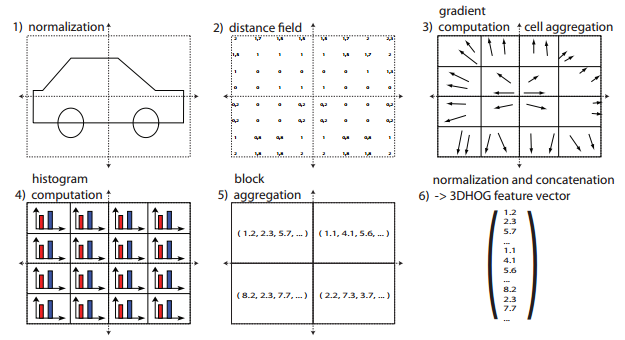
\includegraphics[width=\linewidth]{2-Hauptteil/pics/HOG3D_extrac_pipe.png}
 	\caption{Vektor Extraktionspipeline aus \cite{scherer2010histograms}}
 	\label{Vekt_ext_pipe}
 \end{figure}
 
\subsection{Experiment}
Im folgenden werde ich das in \cite{scherer2010histograms} durchgeführte Experiment und dessen Ergebnisse vorstellen. Um die Effizienz der Deskriptoren zu vergleichen werden Precision-and-recall-Diagramme verwendet

\subsubsection{Verwendete Benchmarks}
Für das Experiment wurden drei etablierte Benchmarks genommen, welche 3D Mesh Modelle enthalten. Princton Shape Benchmark (PSB), 2009 SHREC Generic Shape Retrieval Contest dataset (SHREC) und Konstanz 3D shape database (KN-DB). Die einzelnen 3D Modelle sind in verschiedene Klassen eingeteilt (z.B. Menschen, Tiere, Autos, .. ), damit verschiedene 3D Deskriptoren besser miteinander verglichen werden können. Je nachdem um welche Objektart es sich handelt, liefern Deskriptoren unterschiedlich gute Ergebnisse. 

\begin{table}[H]
	\centering
	\caption{My caption}
	\label{my-label}
	\begin{tabular}{lllll}
		Benchmark & anz. Modelle & anz. Klassen & durchschn. anz. M. pro K. &  \\
		PSB       & 1814         & 92           & 10                                 &  \\
		KN-DB     & 473          & 55           & 9                                  &  \\
		SHREC     & 720          & 40          & 18                                & 
	\end{tabular}
\end{table}
\subsubsection{Verwendete Vergleichsdeskriptoren}
Im folgenden werde ich die Vergleichsdeskriptoren kurz anreißen. Details sind in \cite{dvvra3DModelret} zu finden.

\paragraph{438-dimensional Depth-Buffer Descriptor (DBD438)}
Dieser Deskripter nutzt das aus der Computergrafik bekannte Tiefenpufferverfahren. Nach \cite{scherer2010histograms} gilt dieser Deskriptor als einer der effektivsten.

\paragraph{300-dimensional Silhoutte-based Descriptor(SIL300)}
Der SIL300 arbeitet mit der Zerlegung des 3D Models in 2D Silhouetten 
mit den jeweiligen Achsen (y,z) (z,y) und (x,y).

\paragraph{136-dimensional Descriptor based on Radial Extent function (RSH136) }
Bei diesem Deskriptor wird mit der Ausdehnung von 3D Objekten gearbeitet. Die Objekte werden entlang gegebenen Richtungen(entlang von vorher definierten Strahlen) gemessen.

\paragraph{472-dimensonal Hybrid Descriptor (DSR472) }
Hierbei handelt es sich um einen Hybrid aus den vorigen Deskriptoren. Da hier geschickt die einzelnen Stärken kombiniert werden, ist sogar dem DBD438 überlegen.

\subsubsection{Ergebnisse des Experiment}
Zunächst wurde überprüft, ob sich zur Gradientenberechnung ggf. Gradienten der 2. Ableitung (Formel \ref{Abl_''_Maske}) bessere Ergebnisse liefern.    
\begin{equation}
\label{Abl_''_Maske}
\begin{bmatrix}
1 & 0 & -2 & 0 & 1
\end{bmatrix}
\end{equation}
Da dies der Fall war, wurden alle weiteren Benchmarks mit der 2. Ableitung durchgeführt. Im Vergleich mit den einzelnen Deskriptoren schneidet der HOG3D besser ab. Entsprechend wenig überraschend ist er aber dem Hybrid Deskriptor unterlegen. Dennoch schneidet der HOG3D beim SHREC Benchmark bei einzelenen Klassen besser ab, als der Hybrid. Dies legt nahe, dass der HOG3D wichtige 3D Merkmale erkennt, die den anderen Deskriptoren entgehen \cite{scherer2010histograms}.
\newline
Entsprechende Versuche, in denen der HOG3D mit dem DSR472 kombiniert wurde führten zu einer Performanceverbesserung. Der HOG3D stellt damit einen wertvollen Beitrag zur Verbesserung von 3D Objekterkennungssystemen da \cite{scherer2010histograms}.
